\newpage
\section{Material e Métodos}
\label{sc:metodologia_}



{
Inicialmente, foi realizada uma pesquisa dos diversos modelos e tipos de bateria para análise, com a finalidade de se optar por aquela que tenha maior eficiência nos critérios já mencionados (tamanho, custo e carga energética). Após a aferição de mais de 200 modelos diferentes, foram realizados vários filtros para a seleção destes, resultando na Tabela \ref{tabela:tabela_modelos_bateria_label} que possui vinte e oito modelos.
}


\label{sc:tabela_modelos_bateria}

\begin{table}[htp]
\caption{Tabela modelos de baterias}
\vspace{0.5cm}
\label{tabela:tabela_modelos_bateria_label}
\scalefont{0.6}
\begin{tabular}{|c|c|c|c|c|c|c|c|c|c|c|c|c|}
\hline
\multicolumn{1}{|c|}{\multirow{2}{*}{nº}} & \multicolumn{1}{c|}{\multirow{2}{*}{Marca}} & \multicolumn{1}{c|}{\multirow{2}{*}{Modelo}} & \multicolumn{1}{c|}{\multirow{2}{*}{Química}} & \multicolumn{3}{c|}{Dimensões(mm)} & \multicolumn{1}{c|}{\multirow{2}{*}{Tamanho}} & \multicolumn{1}{c|}{\multirow{2}{*}{Preço}} & \multicolumn{1}{c|}{\multirow{2}{*}{Tensão}} & \multicolumn{1}{c|}{\multirow{2}{*}{mAh}} & \multicolumn{1}{c|}{\multirow{2}{*}{Wh}} & \multicolumn{1}{c|}{\multirow{2}{*}{Custo/wh}} \\ \cline{5-7}
\multicolumn{1}{|c|}{}                           & \multicolumn{1}{c|}{}                       & \multicolumn{1}{c|}{}                        & \multicolumn{1}{c|}{}                                & C          & L         & A         & \multicolumn{1}{c|}{}                                   & \multicolumn{1}{c|}{}                       & \multicolumn{1}{c|}{}                                    & \multicolumn{1}{c|}{}                     & \multicolumn{1}{c|}{}                    & \multicolumn{1}{c|}{}                          \\[2pt] \hline
01                                               & Rontek                                      & RT300AAAB4                                   & Ni-cd                                                & 11         & 44        & 11        & Aaa                                                     & R\$4,98                                     & 1,20                                                     & 300,00                                    & 360,00                                   & 0,009722                                       \\[2pt] \hline 
02                                               & Energy Power                                & AA Ni-mh                                     & Ni-mh                                                & 14,5       & 50,5      & 14,5      & Aa                                                      & R\$8,90                                     & 1,20                                                     & 800,00                                    & 960,00                                   & 0,009271                                       \\[2pt] \hline
03                                               & Energy Power                                & AA Ni-cd                                     & Ni-cd                                                & 14,5       & 50,5      & 14,5      & Aa                                                      & R\$9,50                                     & 1,20                                                     & 1000,00                                   & 1.200,00                                 & 0,007917                                       \\[2pt] \hline
04                                               & Rontek                                      & AA Ni-mh                                     & Ni-mh                                                & 14,5       & 50,5      & 14,5      & Aa                                                      & R\$7,50                                     & 1,20                                                     & 2100,00                                   & 2.520,00                                 & 0,002976                                       \\[2pt] \hline
05                                               & Mox                                         & Aaa                                          & Ni-mh                                                & 14,5       & 50,5      & 14,5      & Aa                                                      & R\$3,80                                     & 1,20                                                     & 2700,00                                   & 3.240,00                                 & 0,001172                                       \\[2pt] \hline
06                                               & Knup                                        & KP-BT9V                                      & Ni-mh                                                & 47         & 20        & 15        & Bat P                                                   & R\$12,00                                    & 9,00                                                     & 450,00                                    & 4.050,00                                 & 0,002963                                       \\[2pt] \hline
07                                               & FLEX                                        & FX-45B1                                      & Ni-mh                                                & 47         & 20        & 15        & Bat P                                                   & R\$28,00                                    & 9,00                                                     & 450,00                                    & 4.050,00                                 & 0,008642                                       \\[2pt] \hline
08                                               & FullyMax                                    & -                                            & LIPO                                                 & 9,5        & 26        & 45        & Lipo M                                                  & R\$15,20                                    & 3,70                                                     & 650,00                                    & 2.405,00                                 & 0,006320                                       \\[2pt] \hline
09                                               & Mox                                         & MO-086B                                      & Ni-cd                                                & 31,5       & 44        & 10,5      & Aaa                                                     & R\$19,00                                    & 3,60                                                     & 700,00                                    & 2.520,00                                 & 0,001428                                       \\[2pt] \hline
10                                               & Rontek                                      & 6RT1800SC-CX                                 & Ni-cd                                                & 131        & 51        & 23        & Bat. G                                                  & R\$54,04                                    & 7,20                                                     & 1800,00                                   & 12.960,00                                & 0,004169                                       \\[2pt] \hline
11                                               & Rontek                                      & 6RT3000SC-CX                                 & Ni-mh                                                & 131        & 51        & 23        & Bat. G                                                  & R\$100,14                                   & 7,20                                                     & 3000,00                                   & 21.600,00                                & XXXX                                           \\[2pt] \hline
12                                               & Rontek                                      & 6LR61                                        & Ni-mh                                                & 48         & 26        & 16        & Bat. P                                                  & R\$18,50                                    & 8,40                                                     & 350,00                                    & 2.940,00                                 & XXXX                                           \\[2pt] \hline
13                                               & Rontek                                      & -                                            & Ni-mh                                                & 2          & 16        & 16        & P. Botão                                                & R\$5,15                                     & 3,60                                                     & 80,00                                     & 288,00                                   & XXXX                                           \\[2pt] \hline
14                                               & Rontek                                      & -                                            & Ni-mh                                                & 42         & 14        & 47        & 4 * Aaa                                                 & R\$9,86                                     & 3,60                                                     & 1300,00                                   & 4.680,00                                 & XXXX                                           \\[2pt] \hline
15                                               & Rontek                                      & -                                            & Ni-cd                                                & 17         & 51        & 57        & 3 * aa                                                  & R\$36,85                                    & 7,20                                                     & 600                                       & 4.320,00                                 & XXXX                                           \\[2pt] \hline
16                                               & FullyMax                                    & -                                            & LIPO                                                 & 7          & 20        & 36        & Lipo P                                                  & R\$14,40                                    & 3,70                                                     & 350,00                                    & 1.295,00                                 & 0,011119                                       \\[2pt] \hline
17                                               & minamoto                                    & LFP803048                                    & LiFePO4                                              & 8          & 30        & 50        & Lipo M                                                  & Orçamento                                   & 3,20                                                     & 800                                       & 2.560,00                                 & XXXX                                           \\[2pt] \hline
18                                               & minamoto                                    & LFP603450                                    & LiFePO4                                              & 6          & 34        & 50        & Lipo M                                                  & Orçamento                                   & 3,20                                                     & 700                                       & 2.240,00                                 & XXXX                                           \\[2pt] \hline
19                                               & minamoto                                    & LFP101945HP                                  & LiFePO4                                              & 10         & 19        & 45        & Lipo M                                                  & Orçamento                                   & 3,20                                                     & 440                                       & 1.408,00                                 & XXXX                                           \\[2pt] \hline
20                                               & minamoto                                    & LFP803048HP                                  & LiFePO4                                              & 8          & 30        & 48        & Lipo M                                                  & Orçamento                                   & 3,20                                                     & 800                                       & 2.560,00                                 & XXXX                                           \\[2pt] \hline
21                                               & minamoto                                    & LFR26650E                                    & LiFePO4                                              & 26         & 65        & 26        & D+                                                      & Orçamento                                   & 3,20                                                     & 3300                                      & 10.560,00                                & XXXX                                           \\[2pt] \hline
22                                               & minamoto                                    & LFR18650E                                    & LiFePO4                                              & 18,2       & 64,5      & 18,2      & D+                                                      & Orçamento                                   & 3,20                                                     & 1500                                      & 4.800,00                                 & XXXX                                           \\[2pt] \hline
23                                               & minamoto                                    & LFR18490E                                    & LiFePO4                                              & 18,2       & 48,5      & 18,2      & Aa                                                      & Orçamento                                   & 3,20                                                     & 1000                                      & 3.200,00                                 & XXXX                                           \\[2pt] \hline
24                                               & minamoto                                    & LFR14500E                                    & LiFePO4                                              & 14,1       & 48,5      & 14,1      & Aa                                                      & Orçamento                                   & 3,20                                                     & 500                                       & 1.600,00                                 & XXXX                                           \\[2pt] \hline
25                                               & minamoto                                    & LFR18650P                                    & LiFePO4                                              & 18,2       & 64,5      & 18,2      & D+                                                      & Orçamento                                   & 3,20                                                     & 1100                                      & 3.520,00                                 & XXXX                                           \\[2pt] \hline
26                                               & minamoto                                    & LFR26650P                                    & LiFePO4                                              & 26         & 65        & 26        & D+                                                      & Orçamento                                   & 3,20                                                     & 2300                                      & 7.360,00                                 & XXXX                                           \\[2pt] \hline
27                                               & minamoto                                    & LP104884                                     & LIPO                                                 & 10         & 48        & 84        & -                                                       & Orçamento                                   & 3,7                                                      & 5000                                      & 18.500,00                                & XXXX                                           \\[2pt] \hline
28                                               & FullyMax                                    & -                                            & LIPO                                                 & 10         & 26        & 45        & Lipo M                                                  & 27,20                                       & 3,7                                                      & 800                                       & 2.960,00                                 & 0,00125                                        \\[2pt] \hline
\end{tabular}
\end{table}



{
Logo após a separação desses vinte e oito modelos, foram realizadas novas pesquisas para delimitar possíveis características que filtrassem novamente os mesmos. Foram consultados os vários Datasheets\footnote{Datasheet é um arquivo digital a qual contém diversas informações técnicas do fabricante sobre um dado componente eletrônico. Sempre as informações mais confiáveis são fornecidas por esses arquivos.} referentes aos modelos de ESP e dos modos de funcionamento, chegando a especificamente cinco modelos que se apresentam como possíveis escolhas finais. Essas baterias serão adquiridas para a realização de experimentos práticos, para assim se chegar a uma conclusão definitiva.
}

{
De modo concomitante, para se chegar a um valor confiável do melhor modelo de bateria, foram realizados diversos testes experimentais, todavia, para efetuar tais testes foi feita uma placa shield, figura \ref{fig:placa_de_testes_01}, para a realização desses experimentos. Foi projetado um circuito, cujo esquemático feito no software Proteus (ver figura \ref{fig:esquematico_placa_de_testes_01}). Este, possui 8 leds que estão ligados em current source com 8 pinos digitais da placa WeMos, que serão controlados por um código fonte anteriormente programado. A placa foi projetada para drenar uma corrente fixa em cada digital I/O do ESP, para assim, aferir o consumo de corrente do chip.
}

\begin{figure}[H]
    \centering
    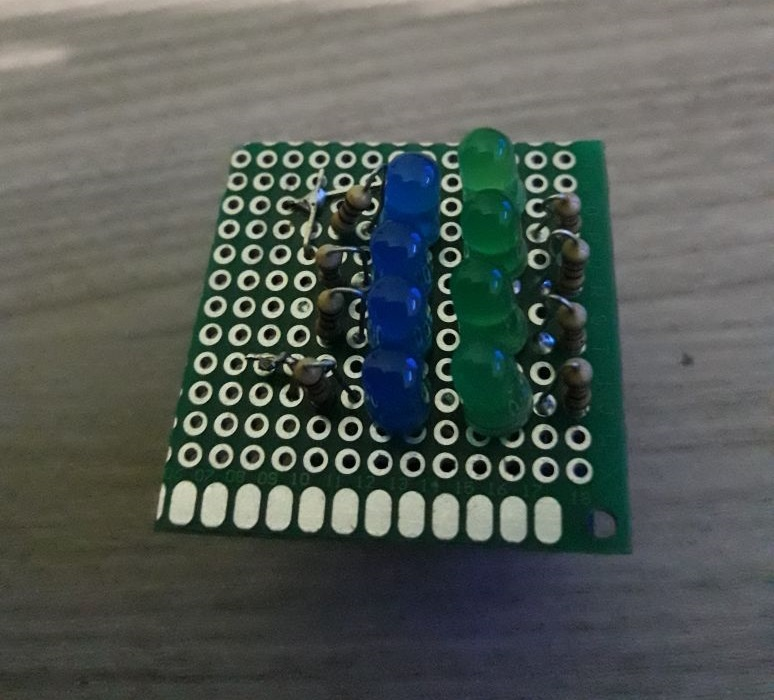
\includegraphics[scale = 0.3]{img/placa_de_testes_01.jpeg}
    \caption{Placa desenvolvida para aferição de consumo do ESP8266}
    \label{fig:placa_de_testes_01}
\end{figure}

\begin{figure}[htp]
    \centering
    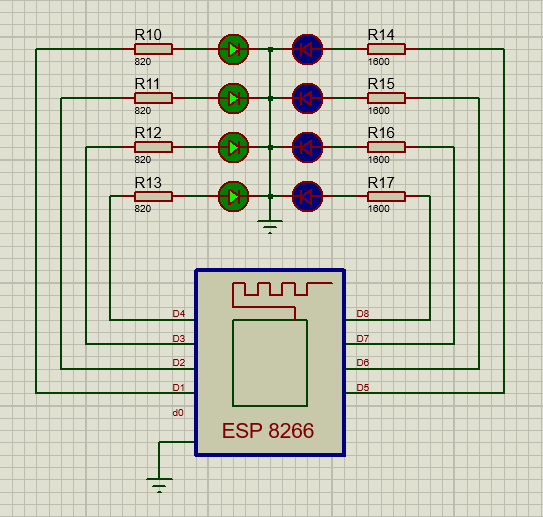
\includegraphics[scale = 0.5]{img/shield_01.png}
    \caption{Esquemático desenvolvido no proteus - Shield 1}
    \label{fig:esquematico_placa_de_testes_01}
\end{figure}

{
Após os primeiros testes de consumo do ESP, foram desenvolvidos diferentes códigos para que se possa aferir o consumo de energia por cada chip em cada modo de operação, modo de transmissão de dados e em cada modo de ‘Sleep\footnote{Sleep é o nome técnico dado ao período em que o processador não realiza grandes funções, como contas aritméticas ou transmissão de dados. Estes períodos de Sleep são utilizados basicamente para se poupar energia, visto que quando o processador entra neste modo, ele não realiza nenhuma operação que demande grande consumo de energia.}’. Cada um desses códigos foi desenvolvido utilizando o Arduino, software IDE, sendo que cada um foi programado utilizando a linguagem C++. Após esta etapa, os códigos foram armazenados, junto aos demais arquivos do projeto, na plataforma Git Hub, com o nome “W8jonas”.
}

{
Ao final da etapa de programação e de aferição do consumo de corrente pela shield 1. Foi feita uma segunda shield, (ver figura \ref{fig:placa_de_testes_02}), capaz d alterar entre os diferentes modos de funcionamento por meio de um botão. O códigoe fonte inserido na placa ESP permite a troca de funções exercidas pelo ESP, desse modo, a cada pressionar do botão, uma nova forma de funcionamento é estabelecida. 
}

\begin{figure}[htp]
    \centering
    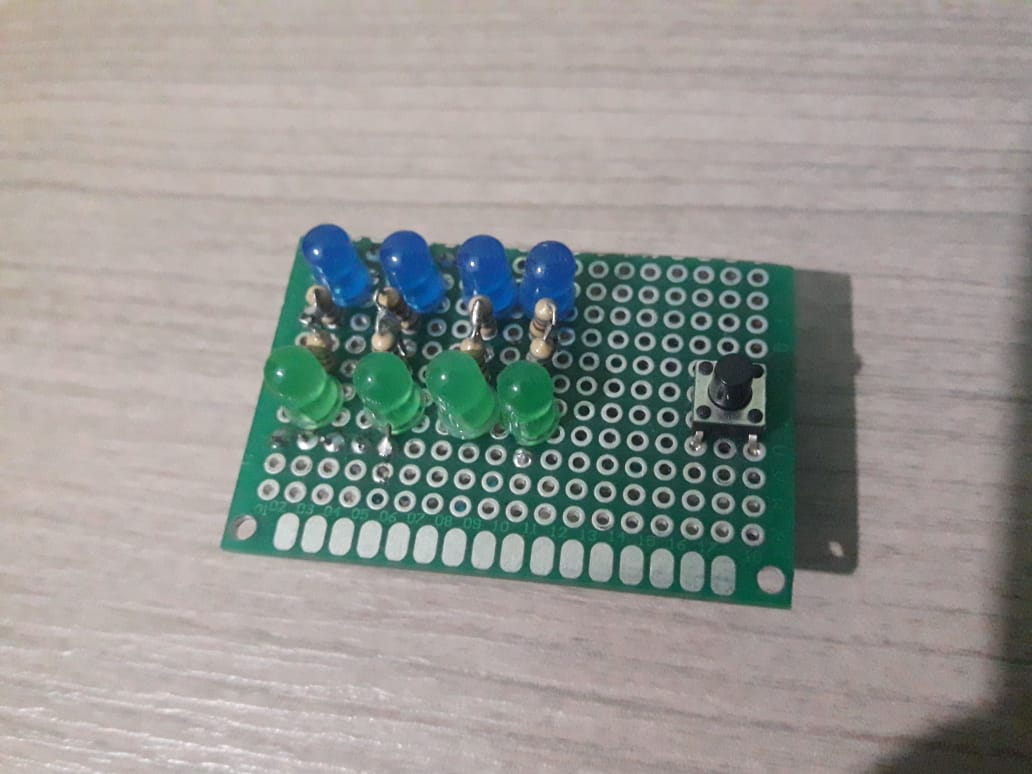
\includegraphics[scale = 0.3]{img/placa_de_testes_02.jpeg}
    \caption{Placa desenvolvida para controlar as funções do ESP}
    \label{fig:placa_de_testes_02}
\end{figure}

{
O código tem como objetivo estabelecer 6 funções diferentes para o Arduino executar cada uma delas de modo separado. Esse programa apresenta dois principais núcleos de funcionamento, a leitura do pressionar do botão, cuja a lógica é compreendida entre as chaves do comando void setup(){ }, e a parte da alteração das funções, em cada função declarada demonstra um modo de funcionamento diferente.
\newline
O código fonte em específico encontra-se na íntegra abaixo:
}

{
\begin{lstlisting}

//  Internet das Vacas código 3
//  Autor: Jonas Henriquee Nascimento
//  PIBIC-Junior
//
//  Data de início: 04/06/2018
//  Data da ultima atualização: 19/06/2018
//  Data de término: 08/06/2018
//  
//  O código tem como objetivo estabelecer 6 funções diferentes para o arduino
//  executar cada uma delas de moto paralelo. Essas funções são escolhidas através 
//  de um botão que toda que apertado faz com que o código execute a função seguinte
//  A primeira função, que é executada junto ao ESP quando é ligado deixa todos os
//  LEDs desligados e o ESP em modo de standby. A segunda função, liga somente um
//  dos LEDs. A terceira, por sua vez, liga todos os 8 LEDs. A próxima função 
//  executa uma série de operações aritméticas, com todos os LEDs desligados. Já a 
//  função 5 executa as mesmas operações aritméticas, mas com 1 dos LEDs ligados. 
//  De tal forma é feito na 6 função, no qual são executadas as operações matemáticas,
//  mas com todos os LEDs ligados.

//  Este código está disponível sempre no endereço abaixo, para livre aperfeiçoamento. 
//  Todavia, pede-se por educação, que ao compartilharem o código, mantenham os autores
//  originais, tão bem quanto o nome da instituição.
//  https://github.com/W8jonas/Internet-das-Vacas/blob/master/programacao/codigo_modos_de_operacao/codigo_modos_de_operacao.ino




#define Output_1 D8
#define Output_2 D7
#define Output_3 D6
#define Output_4 D5
#define Output_5 D4
#define Output_6 D3
#define Output_7 D2
#define Output_8 D1
#define entrada_botao D0

void funcao__();
void funcao_0();
void funcao_1();
void funcao_2();
void funcao_3();
void funcao_4();

int operacao = 0;
boolean leitura = true;

void setup() {
   pinMode (Output_1, OUTPUT);
   pinMode (Output_2, OUTPUT);
   pinMode (Output_3, OUTPUT);
   pinMode (Output_4, OUTPUT);
   pinMode (Output_5, OUTPUT);
   pinMode (Output_6, OUTPUT);
   pinMode (Output_7, OUTPUT);
   pinMode (Output_8, OUTPUT);
   pinMode (entrada_botao, INPUT);
   Serial.begin(115200);
}

void loop() {
  leitura = digitalRead(entrada_botao);
  Serial.println(leitura);
  if (leitura == LOW ){
     operacao++;
     delay(500);
  }

  funcao_2(); 

}

void funcao__ (){
   Serial.println("funcao 00 ");
   digitalWrite(Output_1, LOW);
   digitalWrite(Output_2, LOW);
   digitalWrite(Output_3, LOW);
   digitalWrite(Output_4, LOW);
   digitalWrite(Output_5, LOW);
   digitalWrite(Output_6, LOW);
   digitalWrite(Output_7, LOW);
   digitalWrite(Output_8, LOW);
}

void funcao_0() {
   Serial.println("funcao 0 ");
   digitalWrite(Output_1, HIGH);
}

void funcao_1() {
   Serial.println("funcao 1 ");
   digitalWrite(Output_1, HIGH);
   digitalWrite(Output_2, HIGH);
   digitalWrite(Output_3, HIGH);
   digitalWrite(Output_4, HIGH);
   digitalWrite(Output_5, HIGH);
   digitalWrite(Output_6, HIGH);
   digitalWrite(Output_7, HIGH);
   digitalWrite(Output_8, HIGH);
}

void funcao_2() {
   Serial.println("funcao 2 ");
   digitalWrite(Output_1, LOW);
   digitalWrite(Output_2, LOW);
   digitalWrite(Output_3, LOW);
   digitalWrite(Output_4, LOW);
   digitalWrite(Output_5, LOW);
   digitalWrite(Output_6, LOW);
   digitalWrite(Output_7, LOW);
   digitalWrite(Output_8, LOW);
   int cont = 1;
   float resp = 1;
   float resp2 = 1;
   for(int AA = 0; AA < 500; AA++){
      resp = 3 + sin(resp)/cos(resp*resp/2) * sqrt(sqrt(resp*resp));
      resp = resp * 0.5;
      resp2 = sqrt(AA);
      yield();
  }
}

void funcao_3() {
   Serial.println("funcao 3 ");
   digitalWrite(Output_1, HIGH);
   int cont = 1;
   float resp = 1;
   float resp2 = 1;
   for(int AA = 0; AA < 500; AA++){
      resp = 3 + sin(resp)/cos(resp*resp/2) * sqrt(sqrt(resp*resp));
      resp = resp * 0.5;
      resp2 = sqrt(AA);
      yield();
  }
}

void funcao_4() {
   Serial.println("funcao 4 ");
   digitalWrite(Output_1, HIGH);
   digitalWrite(Output_2, HIGH);
   digitalWrite(Output_3, HIGH);
   digitalWrite(Output_4, HIGH);
   digitalWrite(Output_5, HIGH);
   digitalWrite(Output_6, HIGH);
   digitalWrite(Output_7, HIGH);
   digitalWrite(Output_8, HIGH);
   int cont = 1;
   float resp = 1;
   float resp2 = 1;
   for(int AA = 0; AA < 500; AA++){
      resp = 3 + sin(resp)/cos(resp*resp/2) * sqrt(sqrt(resp*resp));
      resp = resp * 0.5;
      resp2 = sqrt(AA);
      yield();
  }
}

\end{lstlisting}
}

{
Além deste código, foram desenvolvidos outros códigos para o funcionamento de outros modos tratamento de transmissão de sinais, incluindo, também, diferentes formas de economia de energia. Novamente, utilizou-se do pressionar do botão para a alteração entre as funções relativas a cada estado de funcionamento do ESP. Todos os demais códigos feitos encontram-se nos Apêndices deste documento.
}

{
Nesse momento, foram realizadas medidas de consumo de corrente, para isso foram utilizados três multímetros de marcas e modelos diferentes, sendo suas aferições relatadas em maior valor lido e menor valor lido. A tensão foi medida em um resistor shunt de 1 Ω em série com o protótipo de teste de consumo. Após a coleta das seis medidas, foi calculada a média aritmética para se chegar ao resultado final de consumo. A tabela \ref{tabela:tabela_resumo_de_consumo_ESP8266}  apresenta, sucintamente, os valores obtidos, todos os valores medidos, incluindo todas as características dos modos de funcionamento estão dispostos na tabela apresentada no apêndice A.
}


\begin{table}[htp]
\caption{Tabela resumo de consumo ESP8266}
\vspace{0.5cm}
\label{tabela:tabela_resumo_de_consumo_ESP8266}
\begin{tabular}{|l|l|l|}
\hline
Modo de operação                                                     & Configurações do modo      & Consumo médio (mA) \\ \hline
Standby                                                              & VCC = 5v                   & 75,333             \\ \hline
1 Led ligado                                                         & VCC = 5v                   & 75,583             \\ \hline
\begin{tabular}[c]{@{}l@{}}Todos os Leds\\   ligados\end{tabular}    & VCC = 5v                   & 79,3               \\ \hline
100\% uso do CPU                                                     & VCC = 5v                   & 76,9               \\ \hline
\begin{tabular}[c]{@{}l@{}}1 Led ligado + 100\%\\   CPU\end{tabular} & VCC = 5v                   & 77,783             \\ \hline
Todos os Leds + 100\% CPU                                            & VCC = 5v                   & 80,333             \\ \hline
ESP server e cliente ligado                                          & VCC = 5v                   & 75,366             \\ \hline
ESP only client                                                      & VCC = 5v                   & 71,983             \\ \hline
Modem Sleep                                                          & VCC = 5v                   & 71,933             \\ \hline
Light Sleep – CPU ativa                                              & VCC = 5v                   & 16,4               \\ \hline
Light Sleep – CPU desativada                                         & VCC = 5v                   & 2,23               \\ \hline
\multirow{2}{*}{Deep Sleep}                                          & VCC = 5v                   & 0,133              \\ \cline{2-3} 
                                                                     & VCC = 3.3v                 & 0,011              \\ \hline
\multirow{2}{*}{Transmit 802.11b}                                    & VCC = 5v e POUT = +20.5dBm & 75,233             \\ \cline{2-3} 
                                                                     & VCC = 5v e POUT = +14dBm   & 74,866             \\ \hline
\multirow{2}{*}{Transmit 802.11g}                                    & VCC = 5v e POUT = +20.5dBm & 74,050             \\ \cline{2-3} 
                                                                     & VCC = 5v e POUT = +14dBm   & 71,116             \\ \hline
\multirow{2}{*}{Transmit 802.11n}                                    & VCC = 5v e POUT = +20.5dBm & 71,433             \\ \cline{2-3} 
                                                                     & VCC = 5v e POUT = +14dBm   & 71,250             \\ \hline
\end{tabular}
\end{table}

{
Após os valores aferidos, foi feita uma análise de autonomia em relação ao modelo de bateria e aos modos de funcionamento do ESP8266. O padrão de comportamento do chip se apresenta de maneira análoga em todos os casos de análise, pois o funcionamento se baseia em um tempo com o processador ligado, um período com o transmissor de sinais ligado, e um período de Sleep. Esse padrão foi definido dessa forma porque apresenta melhor rendimento.
}

{

}

{
Inicialmente, após a coleta dos dados de consumo, foram criadas equações matemáticas que estimam, de modo aproximado, o gasto energético da placa em diferentes modos de funcionamento com a carga energética das baterias selecionadas, calculando, dessa forma, os valores de autonomia do protótipo. O Gráfico \ref{grafico:grafico_consumo_linear} mostra a relação dos modos de operação selecionados e sua autonomia, tomando como exemplo uma bateria de carga energética igual a 650 mAh. 
}

\begin{figure}[htp]
    \centering
    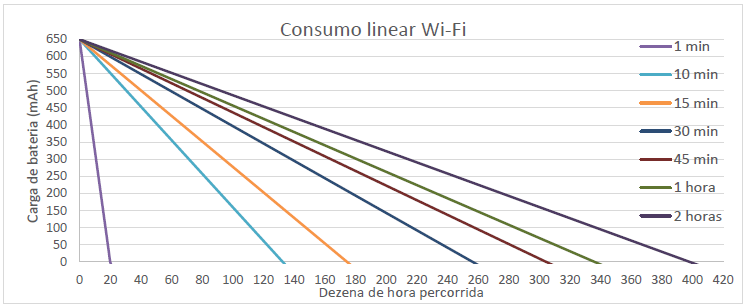
\includegraphics[scale = 0.8]{img/grafico_consumo_linear_prototipo.png}
    \caption{Gráfico consumo linear protótipo 1}
    \label{grafico:grafico_consumo_linear}
\end{figure}

{
Cada modo de operação do Chip possui vantagens e desvantagens, que serão aprimoradas posteriormente junto à codificação final do projeto. Vale salientar que a principal diferença entre os modos está na velocidade dos rastreamentos realizados, sendo que quanto menor o tempo de repetição, mais precisa será a localização. Caso o tempo fosse zero, o monitoramento seria considerado em tempo real, o que se torna possível, mas não viável, pelo alto custo de se manter este sistema funcionando por um longo período.
}

{
A partir das análises preliminares do gráfico, é possível destacar a diferença entre a melhor curva e a pior curva de consumo, destacando, dessa forma, como a pouca diferença entre algumas variáveis altera o resultado final. De certo modo, é impossível que se tenha uma precisão de 100\% no valor de autonomia, isso se deve a dois principais motivos. 
}

{
O primeiro fator se deve a curva de descarga da bateria, a qual não é inteiramente linear, apresentando em seu início e fim curvas exponenciais, dificultando, dessa maneira, os cálculos precisos com relação a descarga da bateria. Essas curvas estão diretamente ligadas aos tipos químicos de cada bateria e os diferentes modelos produzidos por cada empresa da área.
}

{
O segundo fator direciona-se ao fato que os próprios chips possuem variantes internos, estes que por sua vez variam naturalmente, além de serem susceptíveis a variações externas como temperatura. Logo, com variações externas, soma-se as variações resultantes do código fonte executado pelo ESP8266, de suas contas e de suas variações com o decorrer do tempo. Ademais, soma-se as variações de corrente consumida pelo chip em consequência das variações de tensão fornecida pela bateria, visto que esta, ao passar do tempo, tende a diminuir.
}

{
Após os primeiros testes experimentais, foi projetado e montado um circuito capaz de analisar em tempo real os valores de tensão da bateria em decorrer do funcionamento dos chips ESPs em diferentes modelos de bateria. O experimento foi realizado para que se possa aferir divergências entre os valores obtidos teoricamente e os obtidos no funcionamento dos circuitos.
}

{
O funcionamento deste circuito, rotulado de “Circuito datalogger de tensão”, tem como função ler, a cada minuto, o valor de tensão de cada uma das baterias dispostas no circuito que alimentam determinado ESP e armazenar os valores em um arquivo do tipo ‘.svc’ para a análise em algum programa.
}

{
Inicialmente foram gravados os mesmos códigos com suas adaptações tanto para o ESP32 quando para o ESP8266, no qual eram responsáveis por operar o protótipo de modo a seguir o padrão de consumo/funcionamento referente a tabela \ref{tabela:tabela_modos_de_operacao}.
}

\begin{table}[htp]
\caption{Tabela modo de funcionamento}
\vspace{0.5cm}
\label{tabela:tabela_modos_de_operacao}
\scalefont{0.6}
\begin{tabular}{lllllllllll}
\cline{1-4}
\multicolumn{2}{|l|}{Especificações:}                                                                                    & \multicolumn{1}{c|}{Valor}                                    & \multicolumn{1}{c|}{Unidade}                        &                                                     &                                                      &                                                                        &                                                                      &                                                                        &                                                                     &                                                                     \\ \cline{1-4}
\multicolumn{1}{|l|}{}                                            & \multicolumn{1}{l|}{bateria}                         & \multicolumn{1}{l|}{750}                                      & \multicolumn{1}{l|}{mAh}                            &                                                     &                                                      &                                                                        &                                                                      &                                                                        &                                                                     &                                                                     \\ \cline{1-4}
\multicolumn{1}{|l|}{}                                            & \multicolumn{1}{l|}{bateria}                         & \multicolumn{1}{l|}{2700000}                                  & \multicolumn{1}{l|}{mAsec}                          &                                                     &                                                      &                                                                        &                                                                      &                                                                        &                                                                     &                                                                     \\ \cline{1-4}
                                                                  &                                                      &                                                               &                                                     &                                                     &                                                      &                                                                        &                                                                      &                                                                        &                                                                     &                                                                     \\ \hline
\multicolumn{1}{|c|}{Teste}                                       & \multicolumn{1}{c|}{Running}                         & \multicolumn{1}{c|}{Operação}                                 & \multicolumn{1}{c|}{Consumo}                        & \multicolumn{1}{c|}{Tempo de}                       & \multicolumn{1}{c|}{Consumo}                         & \multicolumn{1}{c|}{Consumo}                                           & \multicolumn{1}{c|}{Consumo por}                                     & \multicolumn{1}{c|}{Número de}                                         & \multicolumn{2}{c|}{Duração total}                                                                                                        \\ \cline{10-11} 
\multicolumn{1}{|l|}{(nº)}                                        & \multicolumn{1}{l|}{}                                & \multicolumn{1}{l|}{}                                         & \multicolumn{1}{l|}{(mA)}                           & \multicolumn{1}{l|}{operação (s)}                   & \multicolumn{1}{l|}{(mAsec)}                         & \multicolumn{1}{l|}{por ciclo}                                         & \multicolumn{1}{l|}{hora (mAh)}                                      & \multicolumn{1}{l|}{ciclos possíveis}                                  & \multicolumn{1}{l|}{Em horas}                                       & \multicolumn{1}{l|}{Em dias}                                        \\ \hline
\rowcolor[HTML]{C0C0C0} 
\multicolumn{1}{|c|}{\cellcolor[HTML]{C0C0C0}}                    & \multicolumn{1}{l|}{\cellcolor[HTML]{C0C0C0}Valor X} & \multicolumn{1}{l|}{\cellcolor[HTML]{C0C0C0}Deep Sleep}       & \multicolumn{1}{l|}{\cellcolor[HTML]{C0C0C0}0,133}  & \multicolumn{1}{l|}{\cellcolor[HTML]{C0C0C0}100,00} & \multicolumn{1}{l|}{\cellcolor[HTML]{C0C0C0}13,30}   & \multicolumn{1}{l|}{\cellcolor[HTML]{C0C0C0}}                          & \multicolumn{1}{l|}{\cellcolor[HTML]{C0C0C0}}                        & \multicolumn{1}{l|}{\cellcolor[HTML]{C0C0C0}}                          & \multicolumn{1}{l|}{\cellcolor[HTML]{C0C0C0}}                       & \multicolumn{1}{l|}{\cellcolor[HTML]{C0C0C0}}                       \\ \cline{2-6}
\rowcolor[HTML]{C0C0C0} 
\multicolumn{1}{|c|}{\cellcolor[HTML]{C0C0C0}}                    & \multicolumn{1}{l|}{\cellcolor[HTML]{C0C0C0}Valor Y} & \multicolumn{1}{l|}{\cellcolor[HTML]{C0C0C0}100\% uso do CPU} & \multicolumn{1}{l|}{\cellcolor[HTML]{C0C0C0}76,900} & \multicolumn{1}{l|}{\cellcolor[HTML]{C0C0C0}20,00}  & \multicolumn{1}{l|}{\cellcolor[HTML]{C0C0C0}1538,00} & \multicolumn{1}{l|}{\cellcolor[HTML]{C0C0C0}}                          & \multicolumn{1}{l|}{\cellcolor[HTML]{C0C0C0}}                        & \multicolumn{1}{l|}{\cellcolor[HTML]{C0C0C0}}                          & \multicolumn{1}{l|}{\cellcolor[HTML]{C0C0C0}}                       & \multicolumn{1}{l|}{\cellcolor[HTML]{C0C0C0}}                       \\ \cline{2-6}
\rowcolor[HTML]{C0C0C0} 
\multicolumn{1}{|c|}{\multirow{-3}{*}{\cellcolor[HTML]{C0C0C0}1}} & \multicolumn{1}{l|}{\cellcolor[HTML]{C0C0C0}Valor W} & \multicolumn{1}{l|}{\cellcolor[HTML]{C0C0C0}Transmit 802.11n} & \multicolumn{1}{l|}{\cellcolor[HTML]{C0C0C0}71,433} & \multicolumn{1}{l|}{\cellcolor[HTML]{C0C0C0}5,00}   & \multicolumn{1}{l|}{\cellcolor[HTML]{C0C0C0}357,16}  & \multicolumn{1}{l|}{\multirow{-3}{*}{\cellcolor[HTML]{C0C0C0}1908,46}} & \multicolumn{1}{l|}{\multirow{-3}{*}{\cellcolor[HTML]{C0C0C0}15,26}} & \multicolumn{1}{l|}{\multirow{-3}{*}{\cellcolor[HTML]{C0C0C0}1414,74}} & \multicolumn{1}{l|}{\multirow{-3}{*}{\cellcolor[HTML]{C0C0C0}49,1}} & \multicolumn{1}{l|}{\multirow{-3}{*}{\cellcolor[HTML]{C0C0C0}2,05}} \\
\rowcolor[HTML]{C0C0C0} 
\multicolumn{1}{|l|}{\cellcolor[HTML]{C0C0C0}}                    & \multicolumn{1}{l|}{\cellcolor[HTML]{C0C0C0}}        & \multicolumn{1}{l|}{\cellcolor[HTML]{C0C0C0}POUT = + 20.5dBm} & \multicolumn{1}{l|}{\cellcolor[HTML]{C0C0C0}}       & \multicolumn{1}{l|}{\cellcolor[HTML]{C0C0C0}}       & \multicolumn{1}{l|}{\cellcolor[HTML]{C0C0C0}}        & \multicolumn{1}{l|}{\cellcolor[HTML]{C0C0C0}}                          & \multicolumn{1}{l|}{\cellcolor[HTML]{C0C0C0}}                        & \multicolumn{1}{l|}{\cellcolor[HTML]{C0C0C0}}                          & \multicolumn{1}{l|}{\cellcolor[HTML]{C0C0C0}}                       & \multicolumn{1}{l|}{\cellcolor[HTML]{C0C0C0}}                       \\ \hline
\multicolumn{1}{|c|}{}                                            & \multicolumn{1}{l|}{Valor X}                         & \multicolumn{1}{l|}{Deep Sleep}                               & \multicolumn{1}{l|}{0,133}                          & \multicolumn{1}{l|}{100,00}                         & \multicolumn{1}{l|}{13,30}                           & \multicolumn{1}{l|}{}                                                  & \multicolumn{1}{l|}{}                                                & \multicolumn{1}{l|}{}                                                  & \multicolumn{1}{l|}{}                                               & \multicolumn{1}{l|}{}                                               \\ \cline{2-6}
\multicolumn{1}{|c|}{}                                            & \multicolumn{1}{l|}{Valor Y}                         & \multicolumn{1}{l|}{100\% uso do CPU}                         & \multicolumn{1}{l|}{76,900}                         & \multicolumn{1}{l|}{200,00}                         & \multicolumn{1}{l|}{15380,00}                        & \multicolumn{1}{l|}{}                                                  & \multicolumn{1}{l|}{}                                                & \multicolumn{1}{l|}{}                                                  & \multicolumn{1}{l|}{}                                               & \multicolumn{1}{l|}{}                                               \\ \cline{2-6}
\multicolumn{1}{|c|}{\multirow{-3}{*}{2}}                         & \multicolumn{1}{l|}{Valor W}                         & \multicolumn{1}{l|}{Transmit 802.11n}                         & \multicolumn{1}{l|}{71,433}                         & \multicolumn{1}{l|}{200,00}                         & \multicolumn{1}{l|}{14286,60}                        & \multicolumn{1}{l|}{\multirow{-3}{*}{29679,90}}                        & \multicolumn{1}{l|}{\multirow{-3}{*}{59,36}}                         & \multicolumn{1}{l|}{\multirow{-3}{*}{90,97}}                           & \multicolumn{1}{l|}{\multirow{-3}{*}{12,6}}                         & \multicolumn{1}{l|}{\multirow{-3}{*}{0,53}}                         \\
\multicolumn{1}{|l|}{}                                            & \multicolumn{1}{l|}{}                                & \multicolumn{1}{l|}{POUT = + 20.5dBm}                         & \multicolumn{1}{l|}{}                               & \multicolumn{1}{l|}{}                               & \multicolumn{1}{l|}{}                                & \multicolumn{1}{l|}{}                                                  & \multicolumn{1}{l|}{}                                                & \multicolumn{1}{l|}{}                                                  & \multicolumn{1}{l|}{}                                               & \multicolumn{1}{l|}{}                                               \\ \hline
\end{tabular}
\end{table}


{
O circuito teve como centro o Arduino Mega, a qual serviu de ponte entre a leitura de tensão de cada bateria ligada à um diferente ESP e o armazenamento dessas leituras em um cartão de memória. Para a leitura e o registro serem feitos com sucesso e uma coerente exatidão, foram utilizados dois módulos ao Arduino Mega, o módulo ‘Cartão SD’ e o módulo ‘RTC – Real Time Clock’. Todo seu esquemático pode ser observado na figura \ref{fig:esquematico_datalogger_de_tensao}. Todavia, seu esquemático se apresenta em um nível alto de abstração, visto que os componentes foram representados por meros blocos gráficos, porém, assim, não interferindo na análise do circuito, a partir de seu esquemático.
}

\begin{figure}[H]
    \centering
    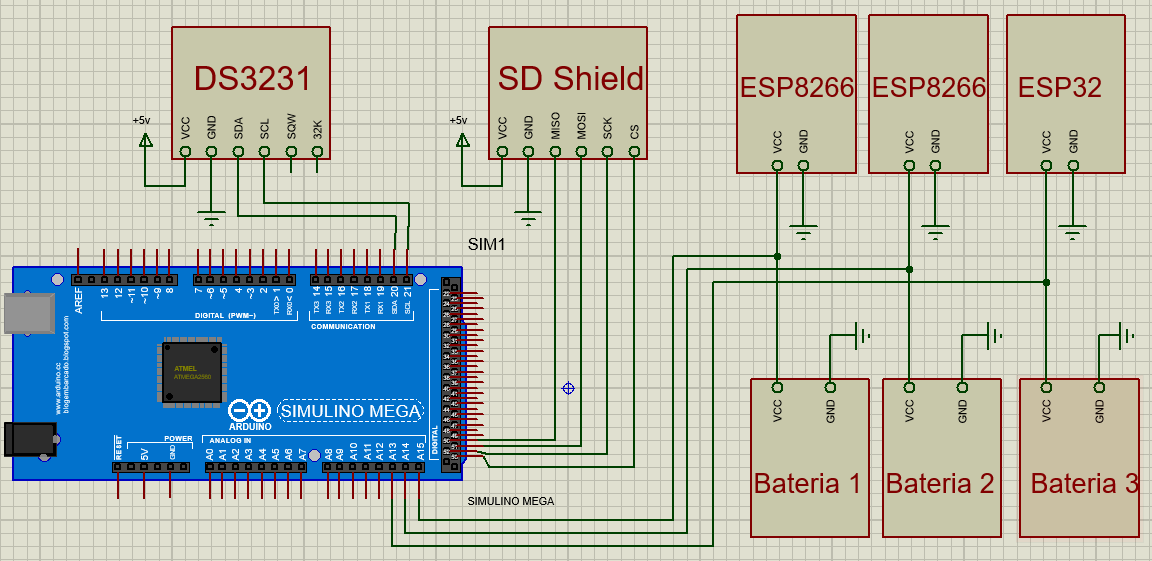
\includegraphics[scale = 0.55]{img/esquematico_datalogger_de_tensao.png}
    \caption{Esquemático do circuito Datalogger de tensão}
    \label{fig:esquematico_datalogger_de_tensao}
\end{figure}

{
Cada um dos módulos teve suas funções bem definidas. O ‘Cartão SD’ foi utilizado para armazenar todos os dados colhidos das leituras, contendo a data e hora da medida, que foram extraídos do RTC. As gravações foram feitas em um arquivo de nome “TENSOEX.SVC”, onde ‘X’ representa o número do teste. Como por exemplo, o teste número 3 teve nome igual a: “TENSOE3.SVC”. 
}

{
Dentro desse arquivo, foram armazenados os dados separados por um caractere indicador, nos primeiros testes, foi escolhido o caractere ‘, ’, porém, após algumas análises, o caractere escolhido foi substituído para ‘; ’. Isso foi feito para que, após o termino das gravações, o arquivo possa ser aberto utilizando algum software para tabulações, o mais conhecido, e que foi utilizado é o Microsoft Excel. A partir dele, é possível abrir esse arquivo e colocar cada valor lido separado em uma célula para posteriormente trabalhar com alguma aplicação no Excel, como a construção de gráficos comparativos. 
}

{
Os dados foram mantidos em uma hierarquização de ordem, em outras palavras, todos os dados foram sempre armazenados na mesma ordem, com a finalidade de se manter um padrão e facilitar a aplicabilidade em diversos programas de tabulação. A ordem escolhida para a escrita no cartão de memória foi: data, hora, valor do sensor 1, valor do sensor 2, erro 1, erro 2, ||; Dessa forma, os dados foram gravados como demonstrado na tabela \ref{tabela:tabela_dados_gravados}:
}


\begin{table}[htp]
\caption{Valores gravados no cartão para análise}
\vspace{0.5cm}
\label{tabela:tabela_dados_gravados}
\scalefont{0.8}
\centering
\begin{tabular}{
>{\columncolor[HTML]{EFEFEF}}l }
\hline
\multicolumn{1}{|c|}{\cellcolor[HTML]{EFEFEF}
11.09.2018; 16:56:00; 3.51; 3.57; 3; 2; ||;} \\ \hline
11.09.2018; 16:57:00; 3.51; 3.56; 3; 2; ||;  \\
11.09.2018; 16:58:00; 3.50; 3.55; 4; 2; ||;  \\
11.09.2018; 16:59:00; 3.50; 3.54; 4; 2; ||;  \\
11.09.2018; 17:00:00; 3.50; 3.53; 4; 2; ||;
\end{tabular}
\end{table}

{
Logo, transcrevendo as informações, temos os dados contidos na tabela \ref{tabela:tabela_dados_contidos_na_gravacao}:
}

\begin{table}[htp]
\caption{Dados contidos na gravação do cartão para análise}
\vspace{0.5cm}
\label{tabela:tabela_dados_contidos_na_gravacao}
\centering
\begin{tabular}{|
>{\columncolor[HTML]{EFEFEF}}l |}
Data: 11.09.2018                            \\
Horas: 16:56:00                             \\
Valor do sensor 1: 3.51                     \\
Valor do sensor 2: 3.57                     \\
Erro 1: 4                                   \\
Erro 2: 2                                   \\
|| : Caractere sinalizador de fim de linha.
\end{tabular}
\end{table}


{
A cada nova leitura de tensão nas baterias, é escrito uma nova linha, logo abaixo do anterior, com a exata mesma sintaxe. Todavia, com seus dados atualizados com os novos valores referentes a leitura. 
}

{
Todo o código fonte pode ser observado abaixo: \newline
}

\begin{lstlisting}

/*
 * Instituto Federal de Educação, Ciência e Tecnologia Minas Gerais
 * IFMG - Campus Avançado Conselheiro Lafaiete 
 * 
 * Internet das Vacas código monitoramento de tensão
 * Autor: Jonas Henrique Nascimento
 * PIBIC-Junior
 * 
 * Data de início.................: 06/09/2018
 * Data da ultima atualização.....: 23/09/2018
 * Data de atualização de versão..: 23/09/2018
 * Data de término................: 23/09/2018
 * 
 * 
 * 
 *  Este código está disponível sempre no endereço abaixo, para livre aperfeiçoamento. 
 *  Todavia, pede-se por educação, que ao compartilharem o código, mantenham os autores
 *  originais, tão bem quanto o nome da instituição.
 *  
 *  https://github.com/W8jonas/Internet-das-Vacas/blob/master/programacao/Monitoramento_de_tensao_2.1/Monitoramento_de_tensao_2.1.ino
 *  
*/


#include <DS3231.h>
#include <SPI.h>
#include <SD.h>
#define chip_select 4


int pino_sensor_de_tensao_ESP32 = A0;             // pino do arduino utilizado para medir a tensao da bateria ligada ao ESP32
float valor_do_sensor_de_tensao_ESP32 = 0;        // variavel de ponto flutuante que armazena o valor de tensao lido do ESP32
                                                  //
int pino_sensor_de_tensao_ESP8266 = A8;           // pino do arduino utilizado para medir a tensao da bateria ligada ao ESP8266
float valor_do_sensor_de_tensao_ESP8266 = 0;      // variavel de ponto flutuante que armazena o valor de tensao lido do ESP8266


int pino_sensor_controle_ESP32 = A1;              // Valor lido de tensao para converter em estado de HIGH ou LOW
float valor_do_sensor_de_controle_ESP32 = 0;      // Valor armazenado de tensao
                                                  //
int pino_sensor_controle_ESP8266 = A9;            // Valor lido de tensao para converter em estado de HIGH ou LOW
float valor_do_sensor_de_controle_ESP8266 = 0;    // Valor armazenado de tensao


unsigned int minuto_antigo = 0;
unsigned int minuto_atual = 0;
unsigned int marcador_tempo_1 = 0;
unsigned int marcador_tempo_2 = 0;

bool flag = false;
bool flag2 = false;
bool flag_controle_marcador_ON = false;
bool flag_controle_marcador_OFF = false;
bool flag_ligado = false;

String texto_marcador = "string marcador";
String dados = "string dados";
String condicao_ = "condicao";

unsigned char erro_marcador_1 = 0;
unsigned char erro_marcador_2 = 0;

void leitura();
void marcador(String marcador);
void gravar_dados_cartao();

DS3231  rtc(SDA, SCL);
Time  t;
File datalogger;

void setup() {
  
   Serial.begin(115200);
   rtc.begin();
   while (!Serial) {;}
   
   if (!SD.begin(chip_select)) {
     Serial.println("Erro ao ler cartao de memoria");
     return;
  }
  
}


void loop() {
   t = rtc.getTime();
   minuto_atual = t.min;
   
   if ( digitalRead(10) == HIGH) {
      condicao_ = "LIGADO";
      marcador(condicao_);
   } else {
      condicao_ = "DESLIGADO";
      marcador(condicao_);
   }
   
   if ( minuto_antigo != minuto_atual ){  
      minuto_antigo = minuto_atual;
      leitura();
      dados = texto_marcador + rtc.getDateStr() + ";" + rtc.getTimeStr() + ";" + valor_do_sensor_de_tensao_ESP8266 + ";" + valor_do_sensor_de_tensao_ESP8266 + ";" + erro_marcador_1 + ";" + erro_marcador_2 + ";*";
      gravar_dados_cartao();
   }

   valor_do_sensor_de_controle_ESP32 = analogRead(pino_sensor_controle_ESP32);
   valor_do_sensor_de_controle_ESP32 =(valor_do_sensor_de_controle_ESP32 * 3.75 ) / 843;
   if(valor_do_sensor_de_controle_ESP32 > 2){
      flag = true;
   }
   if( (valor_do_sensor_de_controle_ESP32 < 1) && (flag == true) ){
      erro_marcador_1++;
      Serial.println("Erro no marcador 2 (ESP32)");
      Serial.println(String (erro_marcador_1));
      Serial.println("  ");
      flag = false;
   }


   valor_do_sensor_de_controle_ESP8266 = analogRead(pino_sensor_controle_ESP8266);
   valor_do_sensor_de_controle_ESP8266 =(valor_do_sensor_de_controle_ESP8266 * 3.75 ) / 843;
   if(valor_do_sensor_de_controle_ESP8266 > 2){
      flag2 = true;
   }
   if( (flag2 == true) && (valor_do_sensor_de_controle_ESP8266 < 1) ) {
      erro_marcador_2++;
      Serial.println("Erro no marcador 1 (ESP8266)");
      Serial.println(String (erro_marcador_2));
      Serial.println("  ");
      flag2 = false;
   }
   
}


void leitura() {
   int x = 0;
   float valor_do_sensor_de_tensao_ESP32_soma = 0;
   float valor_do_sensor_de_tensao_ESP8266_soma2 = 0;
  
   while ( x < 10 ) {
      valor_do_sensor_de_tensao_ESP32 = analogRead(pino_sensor_de_tensao_ESP32);
      valor_do_sensor_de_tensao_ESP32 = (valor_do_sensor_de_tensao_ESP32 * 3.75 ) / 843;
      valor_do_sensor_de_tensao_ESP32_soma = valor_do_sensor_de_tensao_ESP32 + valor_do_sensor_de_tensao_ESP32_soma;
      
      valor_do_sensor_de_tensao_ESP8266 = analogRead(pino_sensor_de_tensao_ESP8266);
      valor_do_sensor_de_tensao_ESP8266 = (valor_do_sensor_de_tensao_ESP8266 * 3.75 ) / 843;
      valor_do_sensor_de_tensao_ESP8266_soma2 = valor_do_sensor_de_tensao_ESP8266 + valor_do_sensor_de_tensao_ESP8266_soma2;
      
      x++;

   }
   valor_do_sensor_de_tensao_ESP32 = valor_do_sensor_de_tensao_ESP32_soma / 10;
   valor_do_sensor_de_tensao_ESP8266 = valor_do_sensor_de_tensao_ESP8266_soma2 / 10;

}


void marcador(String controle){
   if ( (controle == "LIGADO") && (flag_controle_marcador_ON == false) && (flag_ligado == false) ) {
      flag_controle_marcador_ON = true;
      texto_marcador = "\n \n \n \n \n \n \n \n \n \n Data;Hora;valor_do_sensor_de_tensao_ESP32;valor_do_sensor_de_tensao_ESP8266;erro marcador 1 (ESP8266);erro marcador 2 (ESP32); ||; \n";
      flag_ligado = true;
      Serial.println(texto_marcador);
      delay(1000);
   } else {
      if ( (controle == "DESLIGADO") && (flag_controle_marcador_OFF == false) && (flag_ligado == true) ) {
         flag_controle_marcador_OFF = true;
         texto_marcador = "\n \n \n \n \n \n \n \n \n \n  ; ; ; ; ; || \n";
         Serial.println(texto_marcador);
         delay(1000);
      } 
   }
}


void gravar_dados_cartao() {
   
   datalogger = SD.open("2x6.svc", FILE_WRITE);
      if ( datalogger ) {
         Serial.println("Atualizando datalogger");
         Serial.print(dados);
         Serial.println("\n");

         unsigned int tamanho_char = 100;
         char vetor_dados [tamanho_char] = {""};
         dados.toCharArray(vetor_dados, tamanho_char);

         for ( int i = 0; i <= tamanho_char; i++){
            if( vetor_dados[i] == '\n' ){
               datalogger.println(" ");
            }
            if ( vetor_dados[i] == '*' ) {
               break;
            }
            datalogger.write(vetor_dados[i]);
         }
         datalogger.println(" ||;");
         datalogger.close();
      } else {
         Serial.println("Erro ao abrir datalogger");
      }
      Serial.println("Atualizado");
      texto_marcador = "";
      dados = "";
}
\end{lstlisting}


{
Após a leitura dos valores de tensão, foram montados gráficos afim de se analisar o comportamento prático dos primeiros protótipos.
}


